\section {Problem 2}

\begin{figure}[!htb]
    \begin{center}
    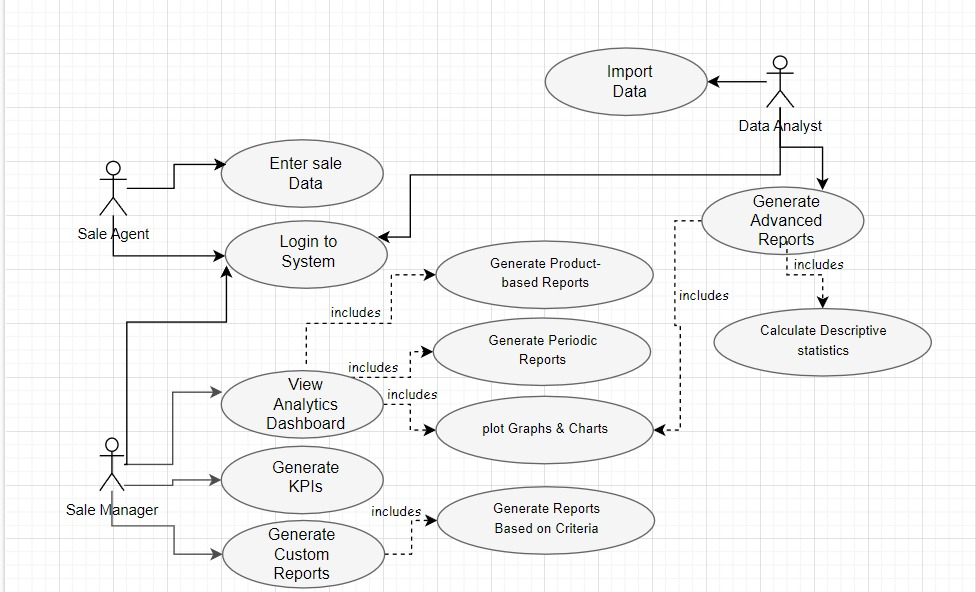
\includegraphics[width=15cm]{images/use_case_diagram.jpeg} % 
    \end{center}
    \caption{Use Case Model \label{Use Case Model}}
\end{figure}

\begin{tabularx}{\textwidth}{|l|X|}
\hline
Use Case ID & UC-1 \\
\hline
Use Case Name & Login to System\\
\hline
Primary Actors & 
\begin{itemize}
    \item Sales Agent
    \item Sales Manager
    \item Data Analyst
\end{itemize} \\
\hline
Priority & High \\
\hline
Description & User can login into the System. \\
\hline
Pre-conditions & 
\begin{itemize}
    \item User has a valid account on the system.
\end{itemize} \\
\hline
Post-conditions & 
\begin{itemize}
    \item User logged in successfully.
\end{itemize} \\
\hline
Scenario & 
\begin{itemize}
    \item User open the login page of the system 
    \item System displays the login page. 
    \item User enters their username and their password. 
    \item User clicks on "Login" button. 
    \item System checks the User’s credentials 	
    \item System displays the homepage.	
    \item User sees the homepage.
\end{itemize}\\
\hline
Exceptional Flow & 
\begin{itemize}
    \item User does not have an account in the system - System notifies user that he/she does not have an account in the system. 
    \item User enters wrong credentials - System notifies user that credentials provided are incorrect.
    \item User is unable to login due to system issues - System logs the problem and provides and error message to the user, suggesting a retry or contact with technical support.
\end{itemize}\\
\hline
\end{tabularx}

\vspace{12pt}

\begin{tabularx}{\textwidth}{|l|X|}
\hline
Use Case ID & UC-2 \\
\hline
Use Case Name & Enter sales Data\\
\hline
Primary Actors & 
\begin{itemize}
    \item Sales Agent
\end{itemize} \\
\hline
Priority & High \\
\hline
Description & User can enter sales data. \\
\hline
Pre-conditions & 
\begin{itemize}
    \item User has a valid account on the system.
    \item There are products in the system.
\end{itemize} \\
\hline
Post-conditions & 
\begin{itemize}
    \item User enters sales data successfully.
\end{itemize} \\
\hline
Scenario & 
\begin{itemize}
    \item User finds product in the system. 
    \item User enters the purchase date, customer information and quantity sold.
    \item User clicks on "Submit" button.
    \item System saves the sales data into the database. 
    \item User is redirected to list of sales data page.
\end{itemize}\\
\hline
Exceptional Flow & 
\begin{itemize}
    \item User is unable to find product in the system - System notifies user that the product does not exist in the system.
    \item User is unable to enter sales data due to system issues - System logs the problem and provides and error message to the user, suggesting a retry or contact with technical support.
\end{itemize}\\
\hline
\end{tabularx}

\vspace{12pt}

\begin{tabularx}{\textwidth}{|l|X|}
\hline
Use Case ID & UC-3 \\
\hline
Use Case Name & View Analytics Dashboard\\
\hline
Primary Actors & 
\begin{itemize}
    \item Sales Manager
\end{itemize} \\
\hline
Priority & High \\
\hline
Description & User can view analytics dashboard which displays product analysis. \\
\hline
Pre-conditions & 
\begin{itemize}
    \item User logs into the system
\end{itemize} \\
\hline
Post-conditions & 
\begin{itemize}
    \item User views analytics dashboard successfully.
\end{itemize} \\
\hline
Scenario & 
\begin{itemize}
    \item User clicks on the "View Analytics Dashboard" button. 
    \item The system displays an analytics dashboard with various performance metrics.
    \item User reviews sales data and KPIs.
\end{itemize}\\
\hline
Exceptional Flow & 
\begin{itemize}
    \item User is unable to view analytics dashboard due to system issues or data retrieval problems - System logs the problem and provides and error message to the user, suggesting a retry or contact with technical support.
\end{itemize}\\
\hline
\end{tabularx}

\vspace{12pt}

\begin{tabularx}{\textwidth}{|l|X|}
\hline
Use Case ID & UC-4 \\
\hline
Use Case Name & Generate Product-based Reports\\
\hline
Primary Actors & 
\begin{itemize}
    \item Sales Manager
\end{itemize} \\
\hline
Priority & Medium \\
\hline
Description & User generate product-based reports based on sales data. \\
\hline
Pre-conditions & 
\begin{itemize}    
    \item User logs into the system
\end{itemize} \\
\hline
Post-conditions & 
\begin{itemize}
    \item User generates product-based reports successfully.
\end{itemize} \\
\hline
Scenario & 
\begin{itemize}
    \item User clicks on the "Generate Product-Based Reports" button. 
    \item The system prompts the user to choose specific products.
    \item The system generates detailed reports on the selected products.
\end{itemize}\\
\hline
Exceptional Flow & 
\begin{itemize}
    \item No data is available for the selected products - System informs the user and suggests alternative products. 
\end{itemize}\\
\hline
\end{tabularx}

\vspace{12pt}

\begin{tabularx}{\textwidth}{|l|X|}
\hline
Use Case ID & UC-5 \\
\hline
Use Case Name & Generate Periodic Reports\\
\hline
Primary Actors & 
\begin{itemize}
    \item Sales Manager
\end{itemize} \\
\hline
Priority & Medium \\
\hline
Description & User can generate periodic reports for sales data. \\
\hline
Pre-conditions & 
\begin{itemize}    
    \item User logs into the system
\end{itemize} \\
\hline
Post-conditions & 
\begin{itemize}
    \item User generates periodic reports for sales data successfully.
\end{itemize} \\
\hline
Scenario & 
\begin{itemize}
    \item User clicks on the "Generate Periodic Reports" button. 
    \item The system prompts the user to specify the reporting period.
    \item The system generates reports summarizing sales data for the chosen trime frame.
\end{itemize}\\
\hline
Exceptional Flow & 
\begin{itemize}
    \item Delay in data processing or issues generating the report - System logs the problem and provides and error message to the user, suggesting a retry or contact with technical support.
\end{itemize}\\
\hline
\end{tabularx}

\vspace{12pt}

\begin{tabularx}{\textwidth}{|l|X|}
\hline
Use Case ID & UC-6 \\
\hline
Use Case Name & Plot Graphs \& Charts\\
\hline
Primary Actors & 
\begin{itemize}
    \item Sales Manager
\end{itemize} \\
\hline
Priority & Medium \\
\hline
Description & User can create visual representations of sales data. \\
\hline
Pre-conditions & 
\begin{itemize}    
    \item User logs into the system
\end{itemize} \\
\hline
Post-conditions & 
\begin{itemize}
    \item User plots graphs and charts for sales data successfully.
\end{itemize} \\
\hline
Scenario & 
\begin{itemize}
    \item User clicks on the "Plot Graphs \& Charts" button. 
    \item The system provides tools to create visual representations of sales data.
    \item User customizes and generate graphs and charts as needed.
\end{itemize}\\
\hline
Exceptional Flow & 
\begin{itemize}
    \item Selected data for visualization contains outliers or incompatible data types - System warns the user and suggests data pre-processing steps. 
\end{itemize}\\
\hline
\end{tabularx}

\vspace{12pt}

\begin{tabularx}{\textwidth}{|l|X|}
\hline
Use Case ID & UC-7 \\
\hline
Use Case Name & Generate KPIs\\
\hline
Primary Actors & 
\begin{itemize}
    \item Sales Manager
\end{itemize} \\
\hline
Priority & Medium \\
\hline
Description & User can calculate and present KPIs based on sales data. \\
\hline
Pre-conditions & 
\begin{itemize}
    \item User logs into the system
\end{itemize} \\
\hline
Post-conditions & 
\begin{itemize}
    \item User can generate KPIs successfully.
\end{itemize} \\
\hline
Scenario & 
\begin{itemize}
    \item User clicks on the "Generate KPIs" button. 
    \item The system calculates and presents key performance indicators (KPIs) based on sales data.
\end{itemize}\\
\hline
Exceptional Flow & 
\begin{itemize}
    \item User is unable to generate KPIs due to errors encountered during KPI calculation because of data inconsistencies or missing values - System logs the problem and provides and error message to the user, suggesting a retry or contact with technical support.
\end{itemize}\\
\hline
\end{tabularx}

\vspace{12pt}

\begin{tabularx}{\textwidth}{|l|X|}
\hline
Use Case ID & UC-8 \\
\hline
Use Case Name & Generate Custom Reports\\
\hline
Primary Actors & 
\begin{itemize}
    \item Sales Manager
\end{itemize} \\
\hline
Priority & Medium \\
\hline
Description & User can customize reports to be generated based on sales data. \\
\hline
Pre-conditions & 
\begin{itemize}
    \item User logs into the system
\end{itemize} \\
\hline
Post-conditions & 
\begin{itemize}
    \item User can generate custom reports successfully.
\end{itemize} \\
\hline
Scenario & 
\begin{itemize}
    \item User clicks on the "Generate Custom Report" button. 
    \item The system provides an intuitive interface for custom report creation.
    \item User defines the report criteria, including date ranges, product categories, and specific metrics of interest.
    \item The system processes the criteria and generates a custom report tailored to the user's specifications.
    \item User reviews and downloads the custom report for further analysis or distribution.
\end{itemize}\\
\hline
Exceptional Flow & 
\begin{itemize}
    \item Criterias are too broad or produces an excessively large report - System notifies the user and suggests refining the criteria for better performance and usability.
    \item Data processing issues or system errors during report generation - System logs the problem and provides and error message to the user, suggesting a retry or contact with technical support.
\end{itemize}\\
\hline
\end{tabularx}

\vspace{12pt}

\begin{tabularx}{\textwidth}{|l|X|}
\hline
Use Case ID & UC-9 \\
\hline
Use Case Name & Generate Reports based on Criteria\\
\hline
Primary Actors & 
\begin{itemize}
    \item Sales Manager
\end{itemize} \\
\hline
Priority & Medium \\
\hline
Description & User can customize reports to be generated based on sales data. \\
\hline
Pre-conditions & 
\begin{itemize}
    \item User logs into the system
\end{itemize} \\
\hline
Post-conditions & 
\begin{itemize}
    \item User can generate custom reports successfully.
\end{itemize} \\
\hline
Scenario & 
\begin{itemize}
    \item User clicks on the "Generate Reports Based on Criteria" button. 
    \item The system provides an intuitive interface for custom report creation.
    \item User defines the report criteria, including date ranges, product categories, and specific metrics of interest.
    \item The system processes the criteria, conducting a targeted analysis based on the user's specifications.
    \item Once the analysis is complete, the system generates a comprehensive report tailored precisely to the provided criteria.
\end{itemize}\\
\hline
Exceptional Flow & 
\begin{itemize}
    \item Criterias are too broad or lead to the generation of an an excessively large report - System notifies the user and suggests refining the criteria for better performance and usability.
    \item Data processing issues or system errors during report generation - System logs the problem and provides and error message to the user, suggesting a retry or contact with technical support.
\end{itemize}\\
\hline
\end{tabularx}

\vspace{12pt}

\begin{tabularx}{\textwidth}{|l|X|}
\hline
Use Case ID & UC-10 \\
\hline
Use Case Name & Import Data\\
\hline
Primary Actors & 
\begin{itemize}
    \item Data Analyst
\end{itemize} \\
\hline
Priority & High \\
\hline
Description & User can import sales data into the system in various formats. \\
\hline
Pre-conditions & 
\begin{itemize}
    \item User logs into the system
\end{itemize} \\
\hline
Post-conditions & 
\begin{itemize}
    \item User imports data successfully.
\end{itemize} \\
\hline
Scenario & 
\begin{itemize}
    \item User clicks on the "Import Data" button. 
    \item The system provides options for uploading various file formats, including CSV, Excel and JSON.
    \item User selected the appropriate file format, file and initiates the import process.
    \item The system parses the data, validates its format and stores it securely within the system database.
    \item Once the import is successful, the user can proceed with using the imported data for further analysis and reporting.
\end{itemize}\\
\hline
Exceptional Flow & 
\begin{itemize}
    \item The uploaded file is incompatible or corrupted - The system notifies the user and suggests using a valid file format or checking the integrity of the uploaded file.
    \item Network issues or system downtimes during data import process - System logs the problem and provides and error message to the user, suggesting a retry or contact with technical support.
\end{itemize}\\
\hline
\end{tabularx}

\vspace{12pt}

\begin{tabularx}{\textwidth}{|l|X|}
\hline
Use Case ID & UC-11 \\
\hline
Use Case Name & Generate Advanced Reports\\
\hline
Primary Actors & 
\begin{itemize}
    \item Data Analyst
\end{itemize} \\
\hline
Priority & High \\
\hline
Description & User can create in-depth analytical reports. \\
\hline
Pre-conditions & 
\begin{itemize}
    \item User logs into the system
\end{itemize} \\
\hline
Post-conditions & 
\begin{itemize}
    \item User generates advanced reports successfully.
\end{itemize} \\
\hline
Scenario & 
\begin{itemize}
    \item User clicks on the "Generate Advanced Reports" button. 
    \item The system provides a user-friendly interface allowing the user to choose from specific data sources, define intricate filters, and choose from a variety of visualization options.
    \item The user configures the report parameters, such as time intervals, comparative metrics and data granularity.
    \item The system processes these parameters, conducts complex data analysis, and generates advanced reports presenting detailed insights and trends derived from the selected data sources.
\end{itemize}\\
\hline
Exceptional Flow & 
\begin{itemize}
    \item The chosen data sources do not contain sufficient data to generate meaningful advanced reports - The system notifies the user and suggests selecting different or additional data sources for analysis.
    \item Issues with visualization tools or rendering engine, resulting in distorted or incomplete reports - System logs the problem and provides and error message to the user, advising the user to adjust the visualization settings or try generating the report again.
\end{itemize}\\
\hline
\end{tabularx}

\vspace{12pt}

\begin{tabularx}{\textwidth}{|l|X|}
\hline
Use Case ID & UC-12 \\
\hline
Use Case Name & Calculate Descriptive Statistics\\
\hline
Primary Actors & 
\begin{itemize}
    \item Data Analyst
\end{itemize} \\
\hline
Priority & High \\
\hline
Description & User can calculate descriptive statistics. \\
\hline
Pre-conditions & 
\begin{itemize}
    \item User logs into the system
\end{itemize} \\
\hline
Post-conditions & 
\begin{itemize}
    \item User calculates descriptive statistics successfully.
\end{itemize} \\
\hline
Scenario & 
\begin{itemize}
    \item User clicks on the "Calculate Descriptive Statistics" button. 
    \item The user specifies a dataset of interest, such as definintg the product sales period, choosing variables and parameters for which descriptive statistics are required.
    \item The system processes this request, performing calculations such as mean, median and standard deviation.
    \item The system generates a detailed report outlining the descriptive statistics of the selected dataset, providing the user with essential insights into the data's central tendencies and variations
\end{itemize}\\
\hline
Exceptional Flow & 
\begin{itemize}
    \item The chosen data sources do not contain sufficient data to generate meaningful advanced reports - The system notifies the user and suggests selecting different or additional data sources for analysis.
    \item Issues with visualization tools or rendering engine, resulting in distorted or incomplete reports - System logs the problem and provides and error message to the user, advising the user to adjust the visualization settings or try generating the report again.
\end{itemize}\\
\hline
\end{tabularx}